\chapter{Diseño} \label{ch:design}
En un proyecto \textit{software}, antes de comenzar a escribir código fuente, se debe
realizar una previa \textbf{elección de modelos en el diseño}, es decir, una elección de
los distintos tipos/modelos de elementos que se quieren usar en la aplicación. Esta elección
nos ayudará en gran medida a la posterior elección de herramientas, explicada en el apartado
\ref{sec:tools}.\\

En los siguientes apartados, se explican y debaten las distintas posibilidades que habría en
la actualidad y por qué usar una u otra. Se desarrollarán los siguientes puntos:

    \begin{enumerate}
        \item Lenguaje nativo o \textit{framework} web (\ref{sec:language-webframework}).
        \item Patrones arquitectónicos de programación (\ref{sec:architectural-patterns}).
        \item Lenguaje CSS nativo o \textit{framework} CSS (\ref{sec:css-frameworkcss}).
        \item Base de datos SQL o base de datos noSQL (\ref{sec:sql-nosql}).
    \end{enumerate}

\section{Lenguaje nativo o \textit{framework} web} \label{sec:language-webframework}
Antes de nada, vamos a explicar brevemente qué es un \textit{framework}. Un
\textbf{\textit{framework}} es un entorno o marco de trabajo que nos ofrece una estructura
base con la que podemos comenzar a elaborar un proyecto. Es una especie de plantilla incial
con la que podremos comenzar y organizar nuestro proyecto \textit{software}. Además, este
permite agilizar mucho el desarrollo, ya que se omiten tareas comunes o repetitivas.\\

Normalmente, cuando se tiene cierta experiencia programando, se van guardando códigos que
se cree que pueden ser útiles en un futuro para ser \textbf{reutilizados}. Por ejemplo, un
sistema de \textit{login} o de registro para una aplicación, ciertas funciones que verifican
estados concretos, etc. Dicho de forma coloquial, estos códigos que vamos creando y
guardando son nuestros \textbf{propios \textit{frameworks}}. Este tipo de \textit{frameworks}
es lo que llamamos código puro, o dicho metafóricamente, escribir código \textit{a pelo},
código escrito directamente sin ayuda de ninguna herramienta. Con esto en mente, ¿por qué
deberíamos usar un \textit{framework} para el desarrollo web? ¿por qué no podríamos usar
nuestros propios \textit{frameworks} simplemente? Pues bien, las razones son sencillas:

    \begin{itemize}
        \item Nuestro código propio nos puede servir a nosotros, pero...¿y a una
        \textbf{tercera persona} que tenga que trabajar en el mismo proyecto?
        \item Si en el proyecto participasen varios programadores y cada uno aportara
        funcionalidades de sus \textit{frameworks} propios, sería muy difícil hacer que todo
        funcionase \textbf{conjuntamente}.
        \item Normalmente, si desarrollamos nuestra propia aplicación sin \textit{frameworks},
        debemos tener en cuenta muchas más consideraciones acerca de la seguridad y
        probablemente tengamos algún \textbf{agujero de seguridad} en nuestro código.
    \end{itemize}

Digamos que un \textit{framework} web es un lugar de trabajo común donde muchos programadores
trabajan en conjunto. Esta es la principal razón por la que muchas empresas buscan
programadores que estén especializados en un \textit{framework} determinado, para que
\textit{hablen el mismo idioma} y puedan resolver tareas y dudas comunes.\\

Como aspectos negativos de usar un \textit{framework} web hay muy pocos, aunque puede
mencionarse que normalmente suele haber modas en las que se usan determinados
\textit{frameworks} más que otros, que pasan a caer en desuso.\\


\section{Patrones arquitectónicos de programación} \label{sec:architectural-patterns}
En la actualidad, existen multitud de patrones arquitectónicos para el desarrollo de
\textit{software}. Dichos patrones definen una forma concreta en la que los componentes
principales de una aplicación se comunican entre sí. Dado que nuestra aplicación tiene una
parte de desarrollo destinada al usuario (\textbf{UI, User Interface}), nos centraremos en
el patrón \textbf{Modelo-Vista-Controlador}.

\subsection{Modelo-Vista-Controlador} \label{sec:mvc}
Es el patrón más común entre los \textit{frameworks}, este se divide en tres bloques:

    \begin{itemize}
        \item \textbf{Modelo}: contiene toda la lógica relacionada con los datos.
        Interacciona de forma habitual con la base de datos mediante operaciones de
        \textbf{selección}, \textbf{inserción}, \textbf{actualización} y \textbf{eliminación}.
        Se comunica con el controlador.
        \item \textbf{Vista}: es la parte visible de la aplicación, es decir, la 
        \textbf{interfaz gráfica} visible al usuario y con la que este interacciona.
        Normalmente está formada por código HTML, CSS y Javascript, y se comunica con el
        controlador.
        \item \textbf{Controlador}: es el punto de unión entre el modelo y la vista. Este
        procesa las \textbf{peticiones (\textit{requests})} que el usuario realiza a través
        de las vistas y las envía al modelo para que este realice las operaciones necesarias
        y genere los datos correspondientes.
    \end{itemize}

El flujo de comunicación entre estos tres bloques es el siguiente:

    \begin{enumerate}
        \item El usuario (navegador) interacciona con la interfaz, generando una petición
        hacia el controlador.
        \item El controlador recibe la petición, la procesa, y la envía hacia el modelo
        si fuese necesario.
        \item Si el controlador ha mandado una petición al modelo, el modelo responde al
        controlador con la información solicitada. 
        \item El controlador manda la información hacia las vistas, que se actualizan con
        dicha información del modelo.
        \item Finalmente, el usuario puede ver las vistas con la información actualizada.
    \end{enumerate}

    \begin{figure}[H]
        \centering
        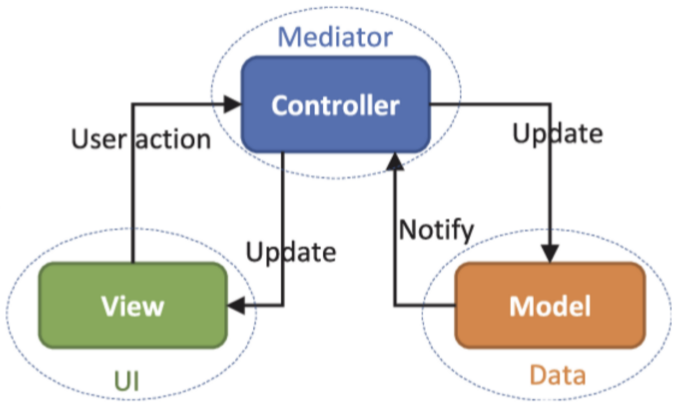
\includegraphics[scale=0.50]{imagenes/mvc.png}
        \caption[Patrón Modelo-Vista-Controlador]{Patrón Modelo-Vista-Controlador. Fuente \cite{mvc}}
        \label{fig:mvc}
    \end{figure}

Dado que vamos a utilizar un \textit{framework} web para el desarrollo de la aplicación, y
la gran mayoría de ellos usan un \textbf{modelo MVC} (\textit{Model-View-Controller}), será
el modelo que utilizaremos. Además, es el patrón con el que más familiarizado estamos.

\section{Lenguaje CSS nativo o \textit{framework} CSS} \label{sec:css-frameworkcss}
Hoy en día, suele haber soluciones \textit{software} para casi todo, y el diseño para la
interfaces de usuario no iba a ser una excepción. Una de las principales razones para usar
un \textit{framework} CSS es el \textbf{incremento de la productividad} durante el desarrollo
de \textit{software}, ya que, al igual que los \textit{frameworks} web, nos proporcionan gran
cantidad de elementos ya definidos como pueden ser componentes, estilos, formularios, etc.
Entre las ventajas de usar un \textit{framework} CSS se encuentran:

    \begin{itemize}
        \item Acelerar la realización de diseños y con ello la productividad.
        \item Posibilitar el trabajo colaborativo, ya que todos los programadores
        trabajan en un mismo marco de trabajo.
        \item Permitir generar un código más limpio y ordenado.
        \item Asegurar la compatibilidad del código fuente entre navegadores.
    \end{itemize}

A pesar de tener muchas cosas buenas, también tiene algunas desventajas, entre las que
podemos mencionar las siguientes:

    \begin{itemize}
        \item Los principios de desacoplamiento entre código HTML y CSS se están perdiendo.
        \item En la mayoría de ocasiones, el \textit{framework} carga gran cantidad de
        código CSS que no se utilizará nunca.
        \item En ocasiones, el usarlo puede llevarnos a desaprender conceptos de CSS que sí
        conocíamos anteriormente.
        \item Al ser \textit{frameworks} usados por miles de usuarios, pueden encontrarse
        páginas muy similares a la desarrollada.
    \end{itemize}

Dadas las ventajas y desventajas que se mencionan, se propone usar código \textbf{CSS nativo}
en combinación con un \textbf{\textit{framework} CSS}, así evitamos algunos de los
inconvenientes como que la página pueda parecerse a otras en la web o que se desaprendan
conceptos de CSS, generando así un balance positivo de su uso.

\section{Base de datos SQL o base de datos noSQL} \label{sec:sql-nosql}
Antes de pasar a la elección de la Base de Datos concreta que vamos a utilizar, necesitamos
tener claro qué \textbf{tipo de base de datos} necesitamos, es decir, usar una base de datos
SQL o una base de datos noSQL. Comencemos dando una breve definición de ambas:
    
    \begin{itemize}
        \item \textbf{Bases de datos relacionales}: son aquellas que utilizan el lenguaje
        SQL (\textit{Structure Query Languaje}), un lenguaje de consulta estructurado. En
        este tipo de bases de datos los elementos se organizan en tablas. Cada fila hace
        referencia a un registro, es decir, a una instancia de esa tabla, mientras que las
        columnas representan campos de esos registros, teniendo un determinado tipo de dato
        cada una. En la actualidad, son el tipo de bases de datos más estándarizado y usado.
        \item \textbf{Base de datos noSQL}: son aquellas bases de datos diseñadas para
        permitir grandes cantidades de datos, tipos de datos complejos, más índices,
        distintos tipos de consulta, etc. En este caso, no existen tablas donde se van
        almacenando los datos, sino que suelen utilizar un esquema clave-valor, documental,
        basado en grafos, etc. Este tipo de base de datos surgió para dar solución a los
        problemas de escalabilidad y rendimiento que las bases de datos relacionales
        generaban al haber miles de usuarios concurrentemente y realizando millones de
        consultas.
    \end{itemize}

En la siguiente tabla se realiza una breve comparación entre ambos tipos: 

    \begin{table}[H]
        \begin{center}
            \begin{tabular}{ |l|l| } \hline
                \textbf{Base de datos SQL} & \textbf{Base de datos noSQL} \\ \hline
                SQL principal lenguaje & SQL como lenguaje de apoyo \\
                Tablas & Hashes, listas \\
                Permite operaciones JOIN & Problemas de rendimiento con JOIN \\
                Escalabilidad vertical & Escalabilidad horizontal \\
                Datos estructurados & Datos menos estructurados \\ 
                Arquitectura centralizada & Arquitectura distribuida \\
                Consistencia & Dinamicidad \\ \hline
            \end{tabular}
            \caption{Tabla con la comparativa entre SQL y noSQL}
            \label{tab:databases}
        \end{center}
    \end{table}

Analizando la naturaleza de nuestro problema, observamos que existen elementos bien
distinguidos en una excavación, como son las \textbf{unidades estratigráficas}, los 
\textbf{hechos}, las \textbf{estancias}, los \textbf{materiales} que se encuentran formando
los hallazgos,....todo ello englobado dentro de las \textbf{excavaciones}. Teniendo esto en
cuenta, habrá datos relacionados entre sí en la aplicación, siendo una de las razones
principales para el uso de una \textbf{base de datos relacional o SQL}. Además, este modelo
es el más utilizado en la actualidad y ninguno de los motivos para el uso de noSQL se da
este proyecto.
